%!TEX root = main.tex
% Legger alt av usability stuff her enn så lenge

% Bruk testplan.docx og test-report.docx som en slags mal til hva som skal være med i plan og rapport. Legg det inn her 
% Se på Usability Master 2 Svanaes.pdf for et forslag til oppsett av dette. F.eks en section med gjennomføring og en med resultater. Slå sammen stuffet fra testplan.docx og test-report.docx til en fin ting!  
\chapter{Usability}
% Her bør vel det nevnes det fra testplanen, kjapt hva vi ville og resultatene stå. Vi bør også forklare testplanen mer et annet sted, såvidt i research method? Men kanskje også reintrodusere test-kapitlet og legge alt fra intro til resultater der? Bør vel ikke stå altfor mye i intro kapitlet dog
% Usability testen er jo ikke den primære evalueringen, men iom. at vi har begrenset med data bør vi nok fokusere litt på den. 
In this section we will describe the results and observations gained through usability tests. Before we conducted the usability test we created a usability test plan: Appendix \ref{chap:usability}, where all the different parts of the usability test is described in detail.
\section{Method}
The usability test was conducted on 5 participants. User-interaction with the PeacefulBanana was done through an Internet Browser. Users answered an entrance questionnaire, in order to collect demographic information. During the usability test we took notes of the user's problems and concerns. When the test was completed, participants could comment with suggestions on improvement of the application or design. Finally we had participants answer a SUS form, which consisted of 10 questions designed to measure user satisfaction. 

\subsection{Context}
The usability test will be using the context and simulate the two scenarios identified in Section \ref{sec:scenarios}. We conduct this usability test in order to answer several important questions, regarding these scenarios: 
\begin{itemize}
	\item Is the application easy to use, and can users achieve their goals in a timely manner?
	\item Identify the relationship users have with the aspect of reflection and sharing personal experiences.
	\item Does the tool present data in a way that triggers reflection for the user?
\end{itemize}
Feedback from the usability test will further aid design and help identify problem areas that might cause problems for potential users. Since the participants are all computer science experts, and are familiar with reflection we hope to receive valuable input regarding these concepts.

\subsection{Test Goals}
The goals of usability testing the PeacefulBanana application include establishing a baseline of user performance, validating user performance measures, and identifying potential design issues that need to be addressed in order to improve efficiency, usability and end-user satisfaction. \\
The usability test objectives are:
\begin{itemize}
	\item Identify possible problems or breakdowns in the design\cite{ref:30} early on in the design process. Sources of such breakdowns may include:
		\begin{itemize}
			\item Navigation errors – failure to locate functions, excessive actions to complete a function, failure to follow recommended screen flow.
			\item Presentation errors – failure to locate and properly act upon desired information in screens, selection errors due to labeling ambiguities.
			\item Control usage problems – improper toolbar or entry field usage.
		\end{itemize}
	\item Exercise the PeacefulBanana application under controlled test conditions with representative users, which here are individuals with a background in IT. Data will be used to assess whether usability goals regarding an effective, efficient, and well-received user interface have been achieved.
	\item Establish baseline user performance and user-satisfaction levels of the user interface for future usability evaluations.
\end{itemize}
The PeacefulBanana application is developed with developers in mind, and will be evaluated on students in the field of Computer Science, developing in an agile team. The testing will occur in a controlled environment in a private room.

Typical problems identified would be text representations or the placement of design elements, that are not intuitive for the user during use. It would be a concern if the user can't figure out how to use certain features of the application. Identifying these problems as early as possible will lead to a better end design. \\
Secondly an objective of the usability test was to identify how users act and think about their daily experiences, how they react to the notion of reflecting on them and if sharing their private thoughts is a problem. 

\subsection{Participants}
As mentioned we had four participants in the usability test. As the PeacefulBanana tool will be used with developers with computer science backgrounds, participants were master students on the Computer Science field at NTNU. These participants all have a background from Computer Science, and is familiar with usability testing and also have experience with the notion of reflection from earlier projects using agile methodologies.
The participants' responsibilities was to attempt to complete a set of representative task scenarios presented to them in as efficient and timely a manner as possible, and to provide feedback regarding the usability and acceptability of the user interface. The participants was directed to provide honest opinions regarding the usability of the application, and to participate in post-session subjective questionnaires and debriefing.

\subsection{Procedure}
The usability test took place in a private room at the university. A computer with the PeacefulBanana web application and supporting software was used in a typical working environment. The participant’s interaction with the application was monitored by the facilitator seated in the same room.
The facilitator briefed the participants on the web application and instruct the participants that we are evaluating the application, rather than evaluating the participant. Participants signed an informed consent that acknowledges: the participation is voluntary, that participation can cease at any time, and that their privacy of identification will be kept safe. \\
The facilitator explained that the amount of time taken to complete the test task will be measured and that exploratory behavior outside the task flow should not occur until after task completion. At the start of each task, the participant read aloud the task description from the printed copy and began the task. Time-on-task measurement began when the participant started the task.
The facilitator instructed the participant to ‘think aloud’ so that the facilitator could observe and take notes of user behavior and user comments.
After all task scenarios are attempted, the participant completed the post-test satisfaction questionnaire.

\subsection{Roles}
For our usability test we had two roles, in addition to the test participants: \\
\subsubsection{Facilitator}
	\begin{itemize}
		\item Provides overview of study to participants.
		\item Defines usability and purpose of usability testing.
		\item Responds to participant's requests for assistance.
	\end{itemize}
\subsubsection{Test Observer}
	\begin{itemize}
		\item Silent observer
		\item Takes notes of identified problems, concerns, coding bugs, and procedural errors.
		\item Serve as note takers.
	\end{itemize}

\subsection{Ethics}
All persons involved with the usability test are required to adhere to the following ethical guidelines:
\begin{itemize}
	\item The performance of any test participant must not be individually attributable. Individual participant's name should not be used in reference outside the testing session.
	\item A description of the participant's performance should not be reported. 
\end{itemize}

\subsection{Usability Tasks}
The usability tasks were derived from our scenarios, described in section \ref{sec:scenarios}. Due to the short time for which each participant was available, the tasks are the most common and relatively complex of available functions. The tasks were identical for all participants in the study.
The application was tested in a development environment and databases were populated during use, and not pre-populated. This ensured a similar experience as to what the users would get when they first use PeacefulBanana in a working setting. The web application was run on a local computer, and not on a dedicated server as it was when deployed in production. This and the possible extra overhead from development mode, may have an impact on performance slightly in a negative way.

\subsubsection{Task context}
PeacefulBanana is a tool intended to promote reflection and allow for revisiting and learning from previous experiences. PeacefulBanana integrates with and collects data from the version-control system Git.
\subsubsection{Scenario 1 tasks:}
Here are the tasks participants were to solve related to Scenario 1:
\begin{itemize}
	\item Task 1: You start the application for the first time, and want to login, link your account with Github and set an active repository.
	\item Task 2: 
		\begin{itemize}
			\item Task 2.1: View your notifications.
			\item Task 2.2: Find the \emph{“Congratulations”} notification and archive it. Find the archive and see if the notification was indeed archived
		\end{itemize}
	\item Task 3:
		\begin{itemize}
			\item Task 3.1: Find the \emph{“Reminder: Daily Reflection”} note and perform the daily summary.
			\item Task 3.2: Find a daily summary note and share it. Verify that is has indeed been shared.
			\item Task 3.3: Find your mood graph
		\end{itemize}
\end{itemize}

\subsubsection{Scenario 2 tasks:}
Here are the tasks participants were to solve related to Scenario 2:
\begin{itemize}
\item Task 4:
	\begin{itemize}
		\item Task 4.1: Create a team with the name \emph{“Tuttifrutti”} and your previously chosen repository.
		\item Task 4.2: Find your created team and set it to active.
		\item Task 4.3: Identify the members on your team and their role.
	\end{itemize}
\item Task 5:
	\begin{itemize}
		\item Task 5.1: Find all your repositories’ milestones.
		\item Task 5.2: Identify your overdue milestones.
		\item Task 5.3: Find your repositories issues.
		\item Task 5.4: Find issue \#17 . Find the status of this issue, when it was opened and when it was closed.
	\end{itemize}
\item Task 6:
	\begin{itemize}
		\item Task 6.1: Generate a tagcloud for your current chosen repository.
		\item Task 6.2: Identify the most used tag for your team and yourself.
		\item Task 6.3: Find the commit impact for your repository.
	\end{itemize}
\end{itemize}

\subsection{Usability Metrics}
Usability metrics refers to user performance measured against specific performance goals necessary to satisfy usability requirements. Scenario completion success rates, error rates, and subjective evaluations was collected. Time-to-completion of scenarios was also collected.

\subsubsection{Scenario Completion}
Each scenario will require, or request, that the participant obtains or inputs specific data that would be used in course of a typical task. The scenario is completed when the participant indicates the scenario's goal has been obtained (whether successfully or unsuccessfully) or the participant requests and receives sufficient guidance as to warrant scoring the scenario as a critical error.
\subsubsection{Critical Errors}
Critical errors are deviations at completion from the targets of the scenario. Obtaining or otherwise reporting of the wrong data value due to participant workflow is a critical error. Participants may or may not be aware that the task goal is incorrect or incomplete.
\subsubsection{Non-Critical Errors}
Non-critical errors are errors that are recovered from by the participant or, if not detected, do not result in processing problems or unexpected results. Although non-critical errors can be undetected by the participant, when they are detected they are generally frustrating to the participant.
\subsubsection{Subjective Evaluations}
Subjective evaluations regarding ease of use and satisfaction will be collected via questionnaires, and during debriefing at the conclusion of the session. The questionnaires will utilize free-form responses and rating scales.
\subsubsection{Scenario Completion Time(time on task)}
The time to complete each scenario, not including subjective evaluation durations, will be recorded.

\subsection{Usability Goals}
The next section describes the usability goals for \emph{PeacefulBanana}
\subsubsection{Completion Rate}
A completion rate of 100\% is the goal for each task in this usability test.
\subsubsection{Error-Free rate}
An error-free rate of 80\% is the goal for each task in this usability test.
\subsubsection{Time on Task(TOT)}
The time to complete a scenario is referred to as "time on task". It is measured from the time the person begins the scenario to the time he/she signals completion.
\subsubsection{Subjective Measures}
Subjective opinions about specific tasks, time to perform each task, features, and functionality will be surveyed. At the end of the test, participants will rate their satisfaction with the overall system. Combined with the interview/debriefing session, these data are used to assess attitudes of the participants.

\subsection{Problem Severity}
To prioritize recommendations, a method of problem severity classification will be used in the analysis of the data collected during evaluation activities. The approach treats problem severity as a combination of two factors - the impact of the problem and the frequency of users experiencing the problem during the evaluation.
\subsubsection{Impact}
\subsubsection{Frequency}
	\begin{itemize}
		\item High: 40\% or more of the participants experience the problem.
		\item Moderate: 20\% - 39\% of participants experience the problem.
		\item Low: 20\% or fewer of the participants experience the problem
	\end{itemize}
\subsubsection{Problem Severity Classification}
	\begin{itemize}
		\item Severity 1: High impact problems that often prevent a user from correctly completing a task. Reward for resolution is reduced redevelopment costs.
		\item Severity 2: Moderate to high frequency problems with moderate to low impact are typical of erroneous actions that the participant recognizes needs to be undone. Reward for resolution is typically exhibited in reduced time on task.
		\item Severity 3: Either moderate problems with low frequency or low problems with moderate frequency; these are minor annoyance problems faced by a number of participants. Reward for resolution is typically exhibited in reduced time on task and increased data
		\item Severity 4: Low impact problems faced by few participants; there is low risk to not resolving these problems. Reward for resolution is typically exhibited in increased user satisfaction.
	\end{itemize}

\section{Usability Test Results}
\subsection{Pilot Test}
After finalizing the usability test plan: Appendix \ref{chap:usability}, a pilot test was conducted prior to the usability-test[ref 22]. The pilot test allows for an evaluation of the test plan itself and the questionaires before doing the actual usability test. This means the pilot test is a "test of the test", where the goal is to evaluate and verify that the test itself is well-formulated. We chose a fellow student as our pilot-tester, in order to check whether the test script was clear, that the tasks were appropriately difficult, and that the data collected can be meaningfully analyzed. 
It also allows the "tester" to practice the execution and guidance, before actually performing the tests. \\
In the pilot test for PeacefulBanana, all of the aspects above were evaluated and a few tweaks were made to the tests, making it more streamlined. Also a few, smaller bugs in the application were discovered and fixed. The test introduction was rewritten, since the pilot-tester showed some confusion in a few of the tasks. 
The findings acted as valuable feedback to our delivery cycle, and were used for improving the design of the application. 
\section{Introduction}
We conducted an onsite usability test using a production version of PeacefulBanana, located on the test administrator’s local server. One tester took notes of comments, facial expressions and navigation choices.The administrator acted as guidance during the test. The sessions captured each participant’s navigational choices, task completion rates, comments, overall satisfaction ratings, questions and feedback.
\section{Executive Summary}
We conducted an onsite usability test at a private lab-room at NTNU on November 10th. The purpose of the test was to assess the usability of the web application design, information flow, information architecture and the effects of sharing personal reflection notes.
Four participants attended the test. Typically, three to five test participants is the optimal number for most usability studies\cite{nielsen1993mathematical}. Each individual session lasted approximately twenty minutes.
% In general ditt og datt , sammendrag av resultatene
This section contains the participant feedback, satisfactions ratings, task completion rates, ease or difficulty of completion ratings, time on task, errors, and recommendations for improvements.
\subsection{Presentation of results}
\subsubsection{Task Completion Success Rate}
\textbf{Scenario 1 completion rates:}
\begin{figure}[h!]
    \centering
        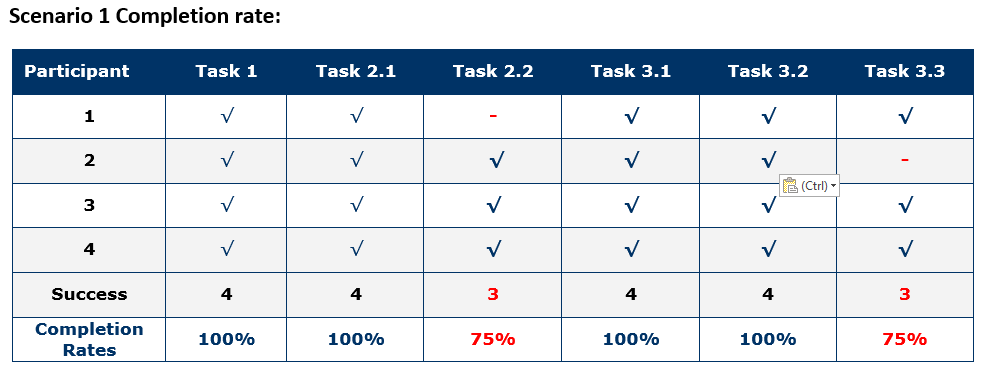
\includegraphics[width=\textwidth]{scenario1completionrate}
    \caption{Scenario 1 Completion Rate}
    \label{scenario1completionrate}
\end{figure}
\begin{figure}[h!]
    \centering
        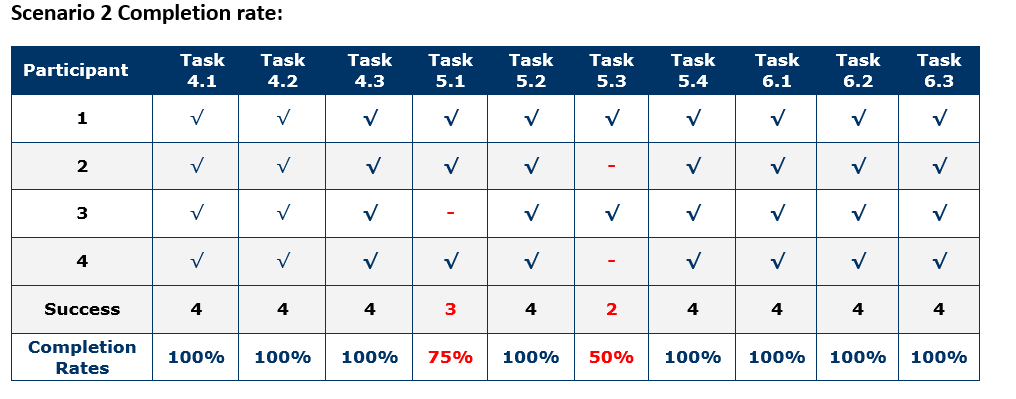
\includegraphics[width=\textwidth]{scenario2completionrate}
    \caption{Scenario 2 Completion Rate}
    \label{scenario2completionrate}
\end{figure}
All participants successfully completed (100\% Completion rate):
\begin{itemize}
	\item Task 1 - Start the application. 
	\item Task 2.1 - View notifications. 
	\item Task 3.1 - Find the \emph{Reminder} note. 
	\item Task 3.2 - Find and share the daily reflection note.
\end{itemize}
For Task 2.2(Find and archive notification) and 3.3(Find mood graph), 3 out of 4 participants completed the tasks(75\% Completion rate). \\

\textbf{Scenario 2 completion rates:}
All participants successfully completed (100\% Completion rate):
\begin{itemize}
	\item Task 4.1 - Create a team. 
	\item Task 4.2 - Set active team. 
	\item Task 4.3 - Identify team members. 
	\item Task 5.2 - Identify overdue milestones. 
	\item Task 5.4 - Find issue \#17
	\item Task 6.1 - Generate tagcloud
	\item Task 6.2 - Identify most used personal tags and team tags
	\item Task 6.3 - Find commit impact
\end{itemize}
3 out of 4 participants(75\%) successfully completed Task 5.1(Find all milestones for your repository), while 2 out 4(50\%) successfully completed Task 5.3 (Find your repositories issues). 

\subsubsection{Time on task}
Time on task for each participant was recorded. Some tasks were inherently more difficult to complete than others and is reflected by the average time on task.
\begin{figure}[h!]
    \centering
        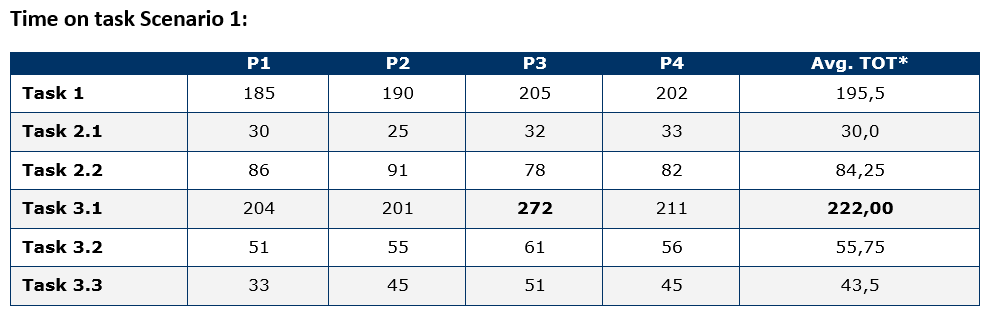
\includegraphics[width=\textwidth]{timeontaskscenario1}
    \caption{Time on task Scenario 1}
    \label{timeontaskscenario1}
\end{figure}
For our tasks in scenario 1, only task 2.2 and Task 3.3
\begin{figure}[h!]
    \centering
        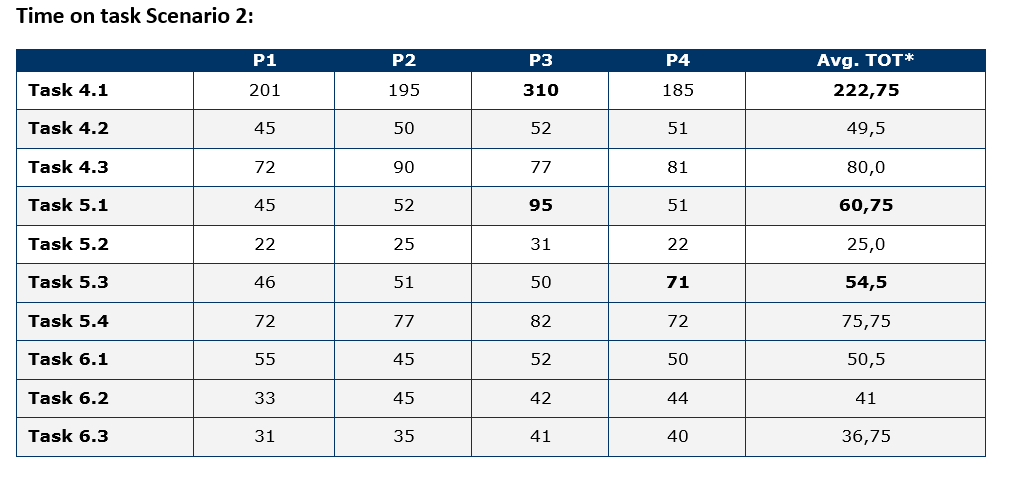
\includegraphics[width=\textwidth]{timeontaskscenario2}
    \caption{Time on task Scenario 2}
    \label{timeontaskscenario2}
\end{figure}
% Skriv litt om de som avviker f.eks: at det tok lenger tid for noen pga de hadde større repo å trekke ned elns 
% Task 6 required participants to find brochures and took the longest time to complete (mean = 210 seconds). However, completion times ranged from 110 (approximately 2 minutes) to 465 seconds (more than 7 minutes) with most times less than 200 seconds (less than 4 minutes). 

\subsubsection{Recommendations}
% Usability test results: Skrive hvordan de svarte på spørsmålene i test-planen, hvordan det gikk. Evt problemer identifisert og at vi da endret disse tingene/designet på bakgrunn av feedbacken. 
% Questionaire resultater:  
% System feedback: Noe om systemet i seg selv.. hvordan det er å bruke, design etc.
% Refleksjonsfeedback: Hvordan var det å skrive ned refleksjonene sine om erfaringene, og hvordan er det å dele de med andre? Mer diagrammer hvis nødvendig. 
